\documentclass{article}

% NeurIPS 2026 GlobalSouthAI workshop, short paper: 4 pages excluding references and appendices, double-blind.
\usepackage[dblblindworkshop]{neurips_2026}
\workshoptitle{GlobalSouthAI}

\usepackage[utf8]{inputenc}
\usepackage[T1]{fontenc}
\usepackage{hyperref}
\usepackage{url}
\usepackage{booktabs}
\usepackage{amsfonts}
\usepackage{amsmath}
\usepackage{nicefrac}
\usepackage{microtype}
\usepackage{xcolor}
\usepackage{graphicx}
\usepackage{multirow}
\usepackage{longtable}

\graphicspath{{figures/}}

% ---- numbers read from data/evaluvation/statutory-qa-v1/ (see paper-numbers.tex) ----
% generated by scripts/statutory-qa/make_paper_numbers.py; do not edit
\newcommand{\nPrincipal}{52}
\newcommand{\nAmending}{60}
\newcommand{\nSections}{4,557}
\newcommand{\nSectionsPrincipal}{4,138}
\newcommand{\nProvisions}{17,854}
\newcommand{\nEdges}{6,346}
\newcommand{\nEdgesDefines}{3,780}
\newcommand{\nEdgesProc}{1,153}
\newcommand{\nEdgesXref}{847}
\newcommand{\nEdgesAmends}{329}
\newcommand{\nEdgesQual}{131}
\newcommand{\nEdgesExc}{106}
\newcommand{\nSectionsAmended}{954}
\newcommand{\corpusFingerprint}{f119236b806f}
\newcommand{\nSourceQ}{667}
\newcommand{\nCandidates}{210}
\newcommand{\nQuarantined}{18}
\newcommand{\nTierB}{66}
\newcommand{\nTierA}{144}
\newcommand{\nTierAMatters}{92}
\newcommand{\nAnnotated}{144}
\newcommand{\nAnnotatedMatters}{92}
\newcommand{\nStatuteOnly}{50}
\newcommand{\nReserved}{38}
\newcommand{\nBlocked}{36}
\newcommand{\nGoldQ}{50}
\newcommand{\nGoldM}{40}
\newcommand{\nGoldEnrich}{25}
\newcommand{\nGoldActs}{23}
\newcommand{\nGoldIndSecs}{84}
\newcommand{\hopOne}{1}
\newcommand{\hopTwo}{10}
\newcommand{\hopThreePlus}{39}
\newcommand{\indOne}{3}
\newcommand{\indTwo}{16}
\newcommand{\indThreePlus}{31}
\newcommand{\nMultiAct}{17}
\newcommand{\nDevM}{8}
\newcommand{\nDevQ}{10}
\newcommand{\nTestM}{32}
\newcommand{\nTestQ}{40}
\newcommand{\nBoot}{2,000}
\newcommand{\cAtTwentyRef}{0.344}
\newcommand{\cAtTwentyOurs}{0.312}
\newcommand{\cAtTenRef}{0.266}
\newcommand{\cAtTenOurs}{0.281}
\newcommand{\rAtTwentyRef}{0.546}
\newcommand{\rAtTwentyOurs}{0.480}
\newcommand{\deltaCTwenty}{-0.031}
\newcommand{\deltaCTwentyLo}{-0.156}
\newcommand{\deltaCTwentyHi}{+0.078}
\newcommand{\actsRetained}{3}
\newcommand{\nSeeds}{15}
\newcommand{\graphWeight}{0.15}
\newcommand{\runName}{main-test}


\title{Does Statutory Structure Help? Retrieving Every Indispensable Provision for Sri Lankan Conveyancing Scenarios}

\author{%
  Anonymous Author(s)\\
  Affiliation\\
  \texttt{email}\\
}

\begin{document}

\maketitle

\begin{abstract}
A conveyancing question is answered only when every provision it turns on is
in hand: the operative rule, the definition it relies on and the exception
that decides the case. We ask whether structure-aware retrieval finds these
complete sets better than flat retrieval does, in Sri Lanka, where prior work
is scored on questions generated from the Act text. We build a corpus of
\nPrincipal{} principal enactments and \nAmending{} amending Acts (\nSections{}
sections, \nEdges{} typed edges for definitions, exceptions, qualifications,
cross-references and amendments); a benchmark of \nGoldQ{} questions in
\nGoldM{} fact patterns from Sri Lanka Law College conveyancing examinations,
each mapped to the sections indispensable to a complete answer with verbatim
provenance; and seven retrievers, from BM25 to a hierarchical system that
routes to Acts, retrieves seed sections and expands them along the typed
edges. The principal metric, complete-indispensable recall, credits a question
only when every indispensable section is retrieved. Structure does not help:
complete recall at 20 is \cAtTwentyRef{} for hybrid BM25 and dense fusion and
\cAtTwentyOurs{} for the structure-aware retriever, with a paired
matter-level bootstrap interval that includes zero. No system completes a
question needing four or more sections, and only two of the sections the
structure-aware retriever missed were reachable by any typed edge from a
retrieved seed: the gold dependencies are jointly required provisions that no
cross-reference wording connects. Gold labels are agent-produced and
agent-verified and are released as proposed gold pending a three-attorney
validation whose protocol we specify.
\end{abstract}

\section{Introduction}

Whether a Sri Lankan notary may attest a deed outside the notary's judicial
zone turns on several provisions at once: the rule limiting territorial
authority, the provision allocating responsibility when two notaries
participate, and the Prevention of Frauds Ordinance provision governing the
validity of notarial execution. Retrieving one or two of them yields an answer
that looks grounded and is legally incomplete, so statutory retrieval should be
judged on whether it returns the complete bundle a question needs.

Legal retrieval benchmarks have mostly scored cases or passages independently
\citep{paul2025ilpcsr, pipitone2024legalbenchrag}. Statute-oriented resources
now pose scenario questions whose facts share little vocabulary with the
controlling text \citep{zheng2025reasoningretrieval}: KoBLEX contains
provision-grounded multi-hop questions \citep{lee2025koblex}, GreekBarRetrieval
pairs bar-examination questions with the articles in official solutions
\citep{greekbarretrieval2026}, and others study structure-aware
\citep{chae2026searchfiresafety} and temporally sensitive
\citep{askingoldfriend2026} statutory retrieval. None jointly separates
indispensable from supporting provisions, scores with an all-or-nothing bundle
measure, and tests through matched ablations whether typed statutory
relationships help. For Sri Lanka, LawChain retrieves over Acts with BM25,
dense embeddings and a Neo4j graph \citep{atukorala2026lawchain}, but its
questions are generated from the legislative text, judged by Gemini, and need
one provision each; \citet{athulathmudali2025rag} retrieve over scenario
records rather than sections; SCaLe-QA \citep{jayawardena2024scaleqa} trains
embeddings on judgments without a section-level benchmark.

We ask: does structure-aware retrieval improve recall of every legally
indispensable provision for scenario questions in a low-resource jurisdiction?
We contribute (1) an expert-informed corpus of Sri Lankan conveyancing and
notarial legislation linking enactments, sections, amending Acts and typed
relationships; (2) a benchmark from sixteen Law College examination papers
whose gold maps separate indispensable, supporting and background provisions
and tie answer claims to verbatim statutory text (\S\ref{sec:data}); and (3)
an evaluation of lexical, dense, hybrid, hierarchical and provision-bundle
retrievers under complete-indispensable recall with matched ablations and
matter-level uncertainty (\S\ref{sec:method}, \S\ref{sec:results}). The
extracted structure does not beat strong hybrid retrieval, because
indispensable provisions are jointly required without any cross-reference
wording connecting them. The gold is agent-produced and agent-verified;
attorney validation has not run, so every number here is a measurement
against proposed gold (\S\ref{sec:limits}).

\section{Corpus and benchmark}
\label{sec:data}

\begin{figure}[t]
  \centering
  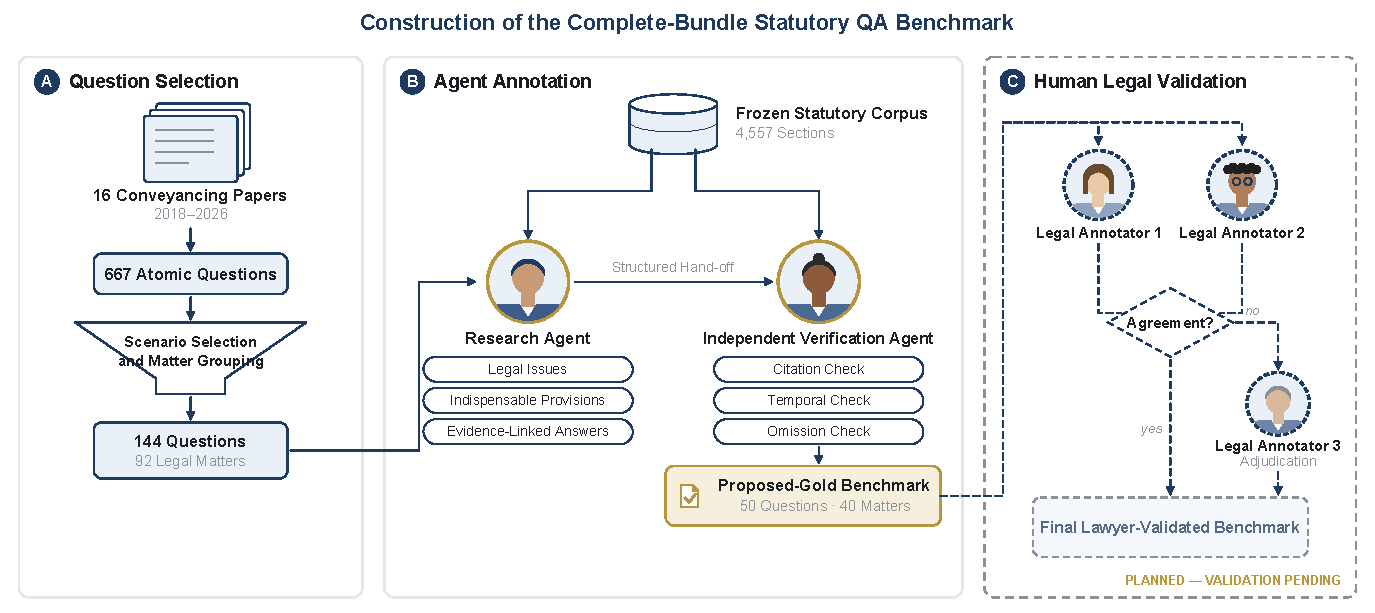
\includegraphics[width=0.68\linewidth]{benchmark-construction.pdf}
  \caption{Benchmark construction. Automated stages (solid) are complete; the
  three-rater legal validation (dashed) is planned and pending.}
  \label{fig:benchmark}
\end{figure}

\paragraph{Corpus.} The principal enactments are the \nPrincipal{} statutes
named in the Sri Lanka Law College conveyancing course tables; we then
collected their amending Acts (Appendix~\ref{app:statutes}). The corpus is
built deterministically from structured JSON trees parsed from Government
Printer and private-republisher PDFs and checked structurally, not legally:
\nPrincipal{} consolidated principal enactments, \nAmending{} amending Acts
kept as separate documents so amendment relationships have a source node,
\nSections{} sections (the retrieval and scoring unit) and \nProvisions{}
sub-section provisions. Six edge types (\nEdges{} edges) are derived from the
trees: cross-references are typed by the wording around them into
\textsc{defines}, \textsc{excepts}, \textsc{qualifies},
\textsc{procedurally\_requires} or \textsc{cross\_references}; a section that
uses a term defined in the same Act gets a \textsc{defines} edge to the
defining section (\nEdgesDefines{} edges, the bulk of the graph);
\textsc{amends} edges link amending sections to the principal sections they
change. Each section carries the year it came into force, which the temporal
filter uses. The cue-word typing is a heuristic and is ablated
(Appendix~\ref{app:corpus}).

\paragraph{Questions and annotation.} We start from \nSourceQ{} atomic
questions split out of sixteen Sri Lanka Law College conveyancing papers (2018
to 2026); \nCandidates{} classified keep or enrich form the candidate pool.
Questions sharing a fact pattern form a matter and are never split across
agents, dataset splits or bootstrap samples. After quarantining
\nQuarantined{} for background-boundary problems and sending \nTierB{} to
manual review, Tier A holds \nTierA{} questions in \nTierAMatters{} matters,
each dated by its exam session so that ``the law in force'' is fixed. Each
matter was researched by one agent (Claude Opus 5, tool access limited to a
search interface over the frozen corpus) and checked by a second agent that
had not seen the research (Figure~\ref{fig:benchmark}). The researcher
classifies the authority requirement (statute only, mixed, case only,
unclear), records every provision with a verbatim excerpt that a validator
checks against the corpus, labels it indispensable, supporting or background,
counts legal hops, drafts an answer with per-claim provenance and, for enrich
questions, adds labelled synthetic facts. The verifier re-reads every cited
section, checks role, temporal applicability and omissions along the corpus
edges, and marks it verified, partially verified, rejected or unresolved. A
question enters the benchmark only if it is
statute-only, every indispensable provision is verified or partially verified,
and the map validates: \nGoldQ{} questions in \nGoldM{} matters, \nGoldActs{}
statutes, \nGoldIndSecs{} distinct indispensable sections, \nMultiAct{}
questions spanning more than one Act, \indThreePlus{} needing three or more
sections (funnel in Appendix~\ref{app:bench}; one record in
Appendix~\ref{app:example}). Questions needing case law are reserved, not
forced into a statute-only answer. The split is by matter: development
\nDevM{} matters (\nDevQ{} questions), test \nTestM{} (\nTestQ{}). Agent
agreement is not legal validation, so the gold is labelled proposed: three
attorneys-at-law will rate independently from the shipped review packets, with
two-of-three agreement on every indispensable provision required for inclusion
(Appendix~\ref{app:bench}); no rating has been collected at the time of
writing.

\section{Retrieval systems}
\label{sec:method}

\begin{figure}[t]
  \centering
  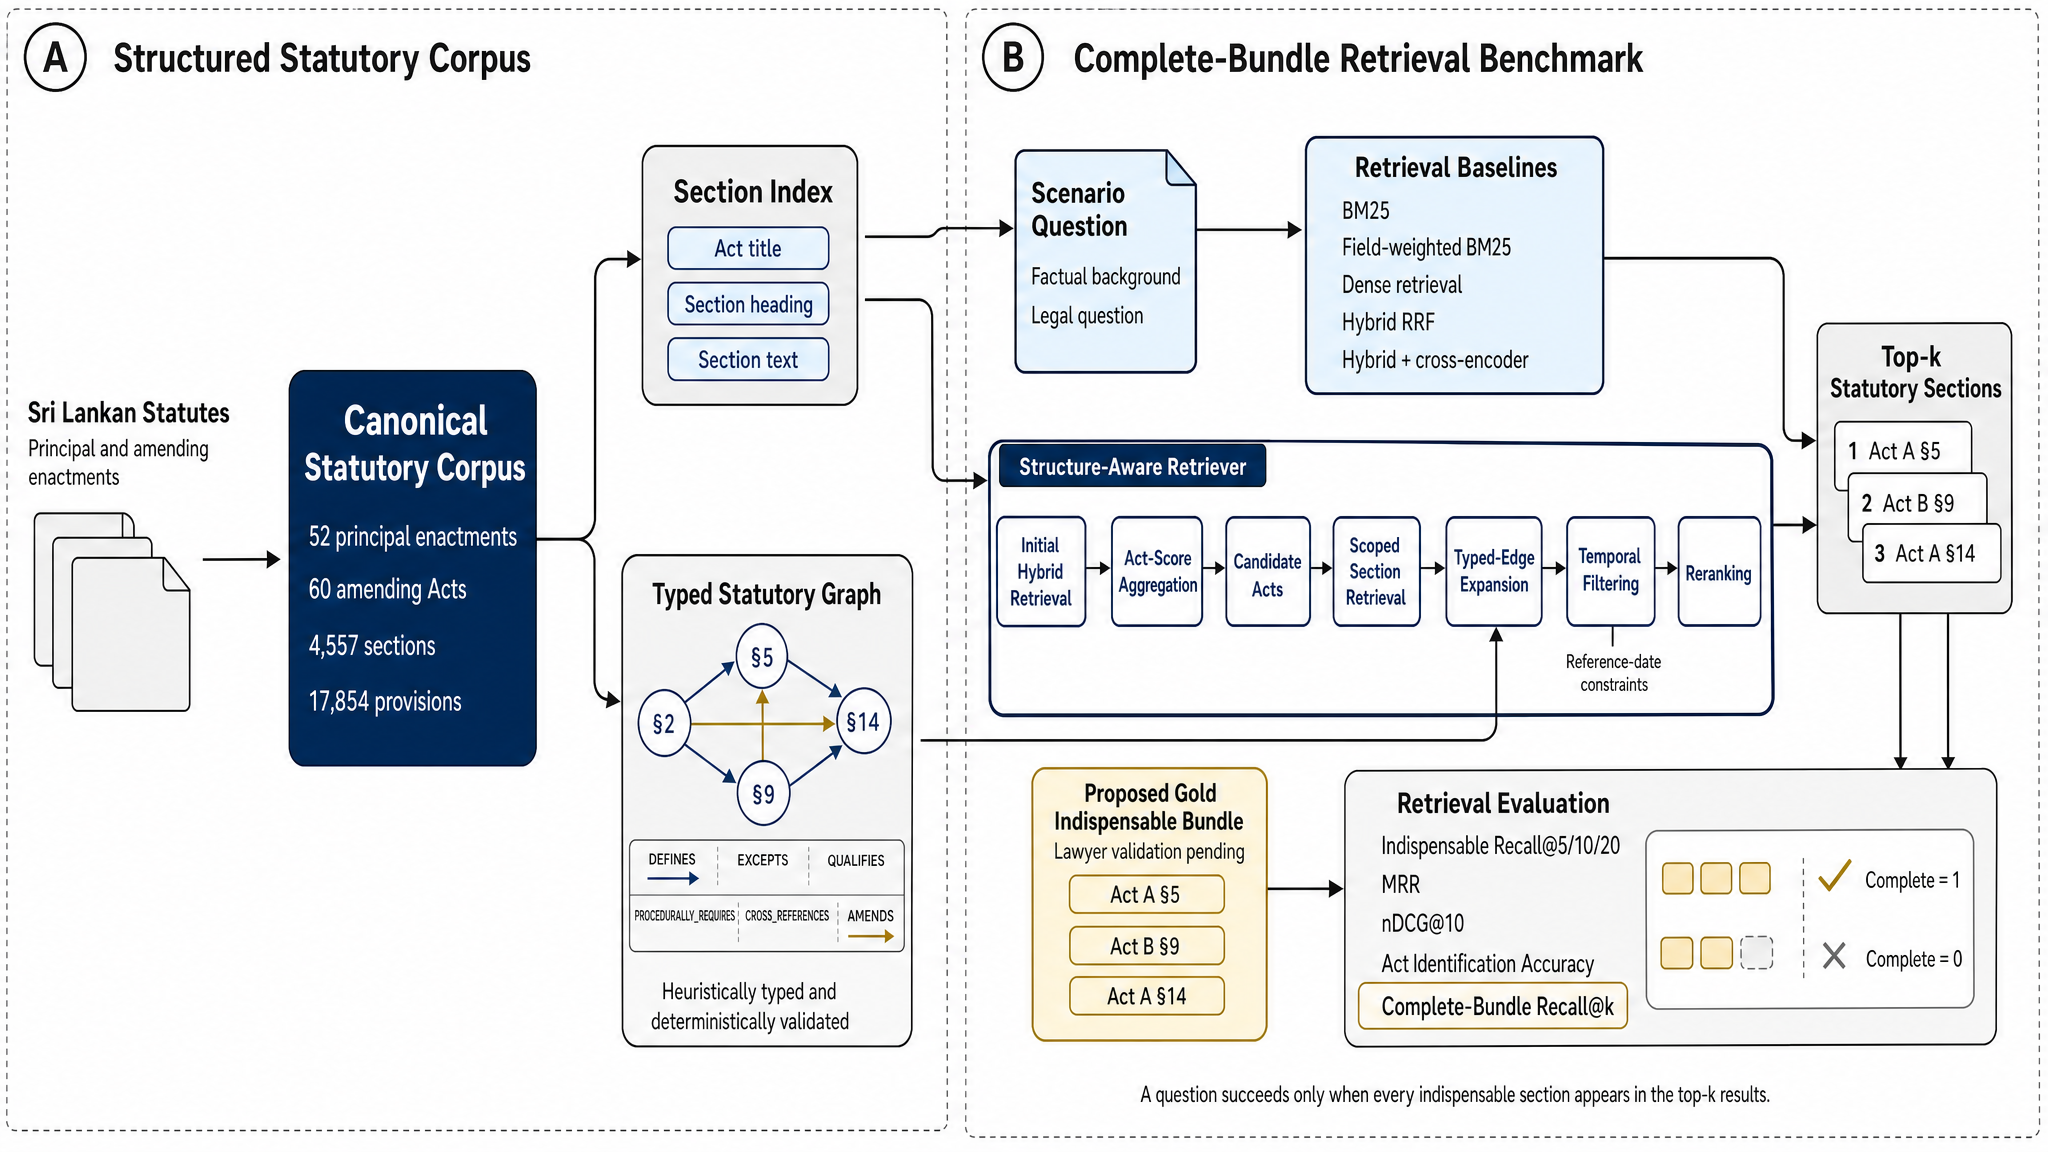
\includegraphics[width=0.68\linewidth]{corpus-retrieval-figure.png}
  \caption{(A) The corpus yields a section index and a typed statutory graph.
  (B) A scenario question is answered by five flat baselines and by the
  structure-aware retriever; the top-$k$ sections are scored against the
  proposed gold bundle, and a question counts only when every indispensable
  section is retrieved.}
  \label{fig:method}
\end{figure}

All systems take the same query, the normalised background (enriched where
enrichment applied) followed by the question, and return sections
(Figure~\ref{fig:method}; settings in Appendix~\ref{app:config}). S1 is BM25
over title, heading and body \citep{robertson2009bm25}. S2 is field-weighted
BM25 over Act title, part heading, section heading, body, defined terms and
cross-reference text. S3 is dense retrieval with \texttt{bge-base-en-v1.5}
\citep{xiao2023bge}, scoring long sections by the maximum over overlapping
windows. S4 fuses S2 and S3 by reciprocal rank fusion \citep{cormack2009rrf}.
S5 reranks the top 100 of S4 with the MS MARCO MiniLM cross-encoder
\citep{wang2020minilm, reimers2019sbert}. S6 follows the document-then-passage
structure of HiREC \citep{choe2025hirec}: Acts are scored by the sum of their
top five fused section scores (amending Acts fold into their principal), the
top \actsRetained{} Acts are kept, and hybrid retrieval is rerun inside them.
S7, the structure-aware retriever, takes the top \nSeeds{} routed sections as
seeds, adds every target of an enabled typed edge to the pool with support
accumulating over seeds, drops sections not in force at the matter's reference
date, reranks with the same cross-encoder, and scores by the average of the
normalised reranker and fused scores plus $\gamma\log(1+\text{support})$,
$\gamma=\graphWeight$. Everything except the reranker and the embedding model
is deterministic, and each component is switched off in turn.

\section{Results}
\label{sec:results}

\paragraph{Metrics.} Indispensable recall at $k$ (R@$k$) is the share of a
question's indispensable sections in the top $k$. Complete-indispensable
recall (C@$k$), the principal metric, is 1 only when all of them are
retrieved, the set-level exact match of KoBLEX \citep{lee2025koblex} at a
cutoff. We also report MRR of the first indispensable section, nDCG@10 (gain 2
indispensable, 1 supporting) and Act identification accuracy at 10. Questions
from one matter are averaged first; means and 95\% intervals are matter-level
bootstraps (\nBoot{} resamples) and comparisons are paired. Hyperparameters
were chosen on the development split; Table~\ref{tab:main} is the test split.

\begin{table}[t]
  \caption{Test split (\nTestQ{} questions, \nTestM{} matters), matter-macro means. R = indispensable recall, C = complete-indispensable recall, Act = Act identification accuracy. Bootstrap intervals in Appendix~\ref{app:ci}.}
  \label{tab:main}
  \centering
  \small
  \begin{tabular}{lccccccc}
\toprule
System & R@10 & R@20 & C@10 & C@20 & MRR & nDCG@10 & Act@10 \\
\midrule
BM25 & 0.452 & 0.491 & 0.250 & 0.281 & 0.503 & 0.345 & 0.719 \\
Field-weighted BM25 & 0.456 & 0.482 & 0.250 & 0.281 & 0.540 & 0.361 & 0.672 \\
Dense (bge-base) & 0.282 & 0.379 & 0.125 & 0.188 & 0.316 & 0.186 & 0.562 \\
BM25F + dense (RRF) & 0.454 & 0.546 & 0.266 & 0.344 & 0.543 & 0.372 & 0.625 \\
Hybrid + cross-encoder & 0.250 & 0.413 & 0.125 & 0.234 & 0.223 & 0.185 & 0.562 \\
Hierarchical Act$\rightarrow$section & 0.447 & 0.496 & 0.297 & 0.375 & 0.509 & 0.357 & 0.469 \\
Hierarchical + bundle (ours) & 0.454 & 0.480 & 0.281 & 0.312 & 0.495 & 0.334 & 0.469 \\
\bottomrule
\end{tabular}

\end{table}

\paragraph{Main result.} Fusing field-weighted BM25 with dense retrieval (S4)
is the strongest system on R@20 (\rAtTwentyRef{}) and on Act identification,
and it ties the hierarchical systems on complete recall: S6 reaches C@20 of
0.375 and S7 \cAtTwentyOurs{}, against \cAtTwentyRef{} for S4, and every
pairwise difference among S4, S6 and S7 has a bootstrap interval that includes
zero (Appendix~\ref{app:ci}). Two components hurt. The web-trained
cross-encoder (S5) drops MRR from 0.543 to 0.223 and C@10 to 0.125. Act
routing with three retained Acts contains every gold Act on only 44\% of test
questions (12 of 40 need two or more Acts), so Act identification falls from
0.625 (S4) to 0.469 (S6, S7), while correctly routed questions are retrieved
more completely, which is why C@20 holds. Dense retrieval alone is weak (C@20
0.188) but lifts BM25 in fusion (R@20 from 0.482 to 0.546). None of this is
comparable with LawChain's recall at 5 of 0.94 \citep{atukorala2026lawchain},
which asks only whether the one source Act of a generated question is in the
top five.

\paragraph{Ablations and errors.} Removing typed expansion, the dense channel,
amendment edges or the reranker from S7 each lowers C@20 by one question in
32 matters; removing definition, exception or cross-reference edges
individually changes nothing; removing the temporal filter gains one question
whose gold is a 2022 amending section that recites superseded wording
(Appendix~\ref{app:ablations}). No difference is separable from zero. Across
systems C@20 is 0.33 to 1.0 on the three test questions with one indispensable
section, 0.25 to 0.67 on the twelve with two, 0.2 to 0.4 on the five with
three, and 0.0 on all twenty with four or more. Of the 114 indispensable
sections S7 left outside its top 20, two were reachable by a single typed edge
from any retrieved seed: the graph is dominated by term-matching definition
edges (\nEdgesDefines{} of \nEdges{}), while the gold dependencies are jointly
required provisions that no cross-reference string connects. Enriched
scenarios, whose added facts name the conditions the provisions test, are
easier than the originals (C@20 0.43 against 0.11 for S7).

\section{Limitations}
\label{sec:limits}

The gold is proposed, not validated. \nBlocked{} Tier A questions were blocked
because the governing text (schedules, stamp duty orders, Roman-Dutch
principles) is not in the corpus and \nReserved{} case-law questions were
reserved, so the benchmark under-represents the hardest questions; the test
split has \nTestM{} matters, so intervals are wide. Edge typing is an
unmeasured cue-word heuristic, temporal filtering uses insertion years rather
than version histories, and answer generation is not scored. The benchmark
measures retrievers, not legal advice: anything scored on it returns
unverified statutory text that a lawyer must check.

\section{Conclusion and future work}
\label{sec:conclusion}

On this benchmark, Act routing and typed-edge expansion as extracted here do
not improve complete recall over hybrid BM25 and dense fusion, and no system
completes a question that needs four or more sections. The gap is coverage,
not ranking: jointly required provisions are rarely joined by cross-reference
wording. Three steps follow. First, complete the three-attorney validation
(Appendix~\ref{app:bench}) and release validated gold with agreement
statistics, so every number here can be re-measured against lawyer-approved
labels. Second, fine-tune the dense retriever and cross-encoder on Sri Lankan
statutory text, since the web-trained reranker halved MRR. Third, widen the
benchmark to the reserved case-law questions, more matters and Acts, and more
systems: query expansion, SPLADE and LLM query rewriting, which the enriched
scenarios suggest matter most.

\bibliographystyle{plainnat}
\bibliography{references}

\appendix

\section{Corpus construction}
\label{app:corpus}

Cross-references are typed by the wording around them: ``within the meaning
of'' becomes \textsc{defines}, ``notwithstanding'' and ``shall not apply''
become \textsc{excepts} (\nEdgesExc{} edges), ``subject to'' becomes
\textsc{qualifies} (\nEdgesQual), ``in the manner prescribed'' and ``under
section'' become \textsc{procedurally\_requires} (\nEdgesProc), and anything
else stays \textsc{cross\_references} (\nEdgesXref). Term-matching
\textsc{defines} edges number \nEdgesDefines{} and \textsc{amends} edges
\nEdgesAmends{}; \nSectionsAmended{} sections have at least one amendment.
\nSectionsPrincipal{} of the \nSections{} sections belong to principal
enactments; provisions are kept for display and gold excerpts. Each section
carries the year it came into force (the Act's year, or the inserting
amendment's). The corpus fingerprint is \texttt{\corpusFingerprint}.

\section{Benchmark funnel and validation protocol}
\label{app:bench}

\begin{table}[h]
  \caption{Benchmark funnel and gold statistics. All gold is proposed and pending lawyer validation.}
  \label{tab:benchmark}
  \centering
  \footnotesize
  \begin{tabular}{lr@{\hskip 1.2em}lr}
    \toprule
    Funnel & questions & Gold set & \\
    \midrule
    source atomic questions & \nSourceQ & questions / matters & \nGoldQ{} / \nGoldM \\
    keep or enrich candidates & \nCandidates & enrich questions & \nGoldEnrich \\
    Tier A (clean, confident) & \nTierA & statutes represented & \nGoldActs \\
    annotated by agents & \nAnnotated & distinct indispensable sections & \nGoldIndSecs \\
    statute-only, proposed gold & \nStatuteOnly & hop count 1 / 2 / 3+ & \hopOne{} / \hopTwo{} / \hopThreePlus \\
    reserved (mixed or case law) & \nReserved & indispensable sections per question 1 / 2 / 3+ & \indOne{} / \indTwo{} / \indThreePlus \\
    blocked (missing authority, ambiguity) & \nBlocked & questions with $>$1 gold Act & \nMultiAct \\
    eligible after verification & \nGoldQ & lawyer approved & 0 \\
    \bottomrule
  \end{tabular}
\end{table}

\paragraph{Annotation checks.} A deterministic validator (no LLM) checks every
legal map against a JSON schema and the corpus: each cited section exists and
its Act, number and title agree with the corpus row; each excerpt is a
verbatim substring of the section body; indispensable, supporting and
background sets are disjoint; a proposed-gold question has at least one
indispensable provision, a hop count of at least one, and no case-law
citation in its answer; enrich questions carry labelled synthetic facts and
keep questions carry none. A verification report and a disagreement log are
written per matter. Review packets and empty approval forms ship with the
data.

\paragraph{Legal validation protocol.} The validation follows the human stage
of KoBLEX \citep{lee2025koblex}, adapted to the provision as the unit. Three
raters, all attorneys-at-law, work independently from the review packets. For
every indispensable provision they answer two questions: is this the correct
authority for the claim it supports, and could the question be answered
completely without it. For every question they answer three more: is the
statute-only classification correct, is any indispensable provision missing,
and how legally accurate is the draft answer on a five-point scale. A question
enters the validated set only when at least two of three raters agree on every
indispensable provision and on statute-only status; disagreements go to
adjudication rather than to a silent majority. We will report raw agreement,
Fleiss' $\kappa$, and the number of agent-proposed provisions rejected, added
or relabelled, which is itself a measurement of agent-produced legal gold.

\section{A benchmark question}
\label{app:example}
One development-split question, rendered from the public-input and
private-gold records. Test-split questions are not printed. Every gold
element below is agent-produced and awaits the validation in
Appendix~\ref{app:bench}.
% generated by scripts/statutory-qa/make_benchmark_example.py; do not edit
\small
\paragraph{Public input.} Question M027-Q01, paper 4, October 2024 sitting; reference date 2024-10; enrichment not applied.
\begin{quote}\small
\textit{Background.} Kanthi Peiris is a Notary practicing in Colombo. Shantha Ratnayake is her brother-in-law and is the owner of an apartment in Negambo. Shantha wishes to lease out his apartment for 3 years at a monthly rental of Rs.120,000/= to one Ananda Gamage who is willing to take on lease in accordance with the said terms. However, Shantha who lives in Negambo is unable to come to Colombo to sign the Agreement.

\textit{Question.} How can this Agreement be signed by both parties and what steps should Kanthi follow with regard to the registration of this Agreement?
\end{quote}
\paragraph{Proposed gold (private view).} Authority requirement \textsc{statute only}; legal hop count 4; gold Acts 1-1907, 23-1927, 7-1840; status \textsc{proposed gold}, lawyer validation \textsc{pending}.
\begin{enumerate}\setlength{\itemsep}{0pt}
\item Whether a three-year lease of an apartment must be executed notarially, and in whose presence the lessor and lessee must sign.
\item How the agreement can be validly signed when the lessor cannot attend before the Colombo notary - execution before more than one notary at different times and places, or execution by a duly authorised attorney under a registered power of attorney.
\item What registration steps the notary must take for a lease of land situated in a district other than the one in which she resides and practises, and within what time.
\end{enumerate}
\begin{tabular}{@{}p{0.30\linewidth}p{0.66\linewidth}@{}}
\toprule Indispensable provision & Excerpt checked verbatim against the corpus \\ \midrule
Prevention of Frauds Ordinance No. 7 of 1840, s.\,2(1)(a) & shall be in force or avail in law unless - (a) the relevant deed or instrument shall be in writing, signed by every executant or by any person duly authorised by such executant and the witnesses in the presence of a lic… \\
Notaries Ordinance No. 1 of 1907, s.\,31 rule (12) & (12) He shall not authenticate or attest any deed or instrument unless the person executing the same and the witnesses shall have signed the same in his presence and in the presence of one another, and unless he shall h… \\
Notaries Ordinance No. 1 of 1907, s.\,31 rule (22) & (22) He shall not authenticate or attest any deed or instrument in any area other than that in which he is authorized to practice, nor in any language other than that in which he is authorized to practice nor authentica… \\
Notaries Ordinance No. 1 of 1907, s.\,31 rule (25) & (25) Where any deed or instrument is executed or acknowledged before more than one notary- (a) the notary who first attests such deed or instrument shall comply with all the requirements of rule (20), and every other no… \\
Notaries Ordinance No. 1 of 1907, s.\,32(2)(i) & (2) In the case of any deed or instrument which is to be executed by two or more parties, both or all of whom, as the case may be, do not sign the deed or instrument at the same time and place- (i) the deed or instrumen… \\
Notaries Ordinance No. 1 of 1907, s.\,31 rule (30A) & (30A) It shall be the duty of every notary to submit for registration to the Registrar, every deed or instrument attested by him before the expiry of thirty days from the date of attestation thereof: Provided that, wher… \\
Registration of Documents Ordinance No. 23 of 1927, s.\,8(b) & (b) if executed or made after the commencement of this Ordinance, all instruments, including wills, decrees and orders of any court or authority, and awards, which purport or operate to create, confer, declare, limit, a… \\
Registration of Documents Ordinance No. 23 of 1927, s.\,14(1) & (1) Every instrument presented for registration shall be registered in the book allotted to the division in which the land affected by the instrument is situated \\
Notaries Ordinance No. 1 of 1907, s.\,2 & Every appointment to the office of notary shall be by warrant granted by the Minister, and shall specify the area within which, and the language or languages in which, the person appointed is authorized to practice. \\
\bottomrule\end{tabular}

\noindent Supporting (not scored): 1-1907/s37, 23-1927/s26, 23-1927/s7, 4-1902/s2, 4-1902/s3, 4-1902/s3A, 4-1902/s3B.

\noindent Reasoning edges (source $\to$ target):

\noindent\begin{tabular}{@{}lp{0.74\linewidth}@{}}
\textsc{jointly required} & 7-1840/s2 $\to$ 1-1907/s31; 23-1927/s8 $\to$ 23-1927/s14 \\
\textsc{qualifies} & 1-1907/s31 $\to$ 1-1907/s32; 23-1927/s8 $\to$ 23-1927/s7 \\
\textsc{procedurally requires} & 7-1840/s2 $\to$ 1-1907/s31; 1-1907/s31 $\to$ 23-1927/s14 \\
\textsc{cross references} & 1-1907/s31 $\to$ 4-1902/s2; 4-1902/s3A $\to$ 7-1840/s2 \\
\textsc{defines} & 1-1907/s2 $\to$ 1-1907/s31 \\
\end{tabular}
\paragraph{Draft answer (agent-written, unvalidated).}
\textit{Issue.} How a three-year lease of a Negombo apartment at Rs.120,000 a month can be signed by a lessor who cannot come to Colombo and by a lessee who can, and what a Colombo notary must then do to register the instrument.

\textit{Rule.} A lease of immovable property for a period exceeding one month is of no force in law unless it is in writing, signed by every executant, or by a person duly authorised by the executant, and by the witnesses in the presence of a licenced notary present at the same time and in the presence of one another, and attested by that notary (Prevention of Frauds Ordinance s.2(1)(a)). The notary may not attest unless the executant and the witnesses signed in her presence and in the presence of one another (Notaries Ordinance s.31 rule (12)), and she may not attest in any area other than the area in which she is authorised to practise (s.31 rule (22)). The Ordinance nevertheless contemplates a deed executed or acknowledged before more than one notary and divides the attestation duties between the first attesting notary and every other attesting notary (s.31 rule (25)), and s.32(2) provides for parties who do not sign at the same time and place, deeming the instrument executed for the purposes of rules (6), (7), (23) and (25) when it is first signed. Alternatively the lessor may authorise an attorney: a power of attorney executed in Sri Lanka must be executed before two witnesses and attested by a notary (Powers of Attorney Ordinance s.2), must meet the additional requirements of s.3A where the transaction falls within s.2 of the Prevention of Frauds Ordinance, must be submitted for registration with the Registrar-General within one month (s.3(1)(b)), and the attesting notary must check the Registrar-General's volumes and folios and state in her attestation that it has not been revoked (s.3B), keep a true copy with her protocol and forward a copy with the duplicate (Notaries Ordinance s.31 rule (30)), and take the attorney's affidavit that the power is genuine, in force and the grantor alive. As to registration, an instrument creating an interest in land is deemed to affect land and so is registrable (Registration of Documents Ordinance s.8(b)), an unregistered instrument is void against a subsequent duly registered instrument taken for value (s.7(1)), registration must be effected in the book allotted to the division in which the land is situated (s.14(1)), and the notary acting for a party may present it (s.26(1)(d)). The notary must submit the deed for registration within thirty days of attestation, or sixty days where it is to be registered outside the jurisdiction in which she practises (Notaries Ordinance s.31 rule (30A)), send the duplicate and Form F1 list to the Registrar of Lands of her own district by the fifteenth of the following month (rule (26)), send a certified copy to the Registrar of Lands of the district where the land lies (rule (29)), and use due diligence in registering where she has instructions and funds (s.37).

\textit{Application.} The lease is for three years, well outside the one-month exclusion, so notarial execution is compulsory and Shantha cannot simply sign at home and send the paper to Colombo. Kanthi practises in Colombo and the apartment and Shantha are in Negombo, so rule (22) prevents her attesting Shantha's signature outside the area she is authorised for. Two lawful routes remain. First, execution before more than one notary under rule (25): Ananda Gamage signs the agreement before Kanthi in Colombo with two witnesses, and Shantha signs the same instrument before a notary authorised to practise where he is, each notary attesting the signatures taken before her or him, each numbering the instrument in his or her own protocol register, and s.32(2) accommodating the fact that the parties sign at different times and places. Second, Shantha grants a power of attorney, attested by a notary before two witnesses and complying with s.3A because the lease falls within s.2 of the Prevention of Frauds Ordinance, registers it with the Registrar-General within one month, and his attorney then signs before Kanthi in Colombo along with Ananda; Kanthi must satisfy herself from the Registrar-General's volumes and folios that the power stands unrevoked and say so in her attestation, take the attorney's affidavit, and keep and forward copies of the power. Either way she must have an assurance that the stamp duty is provided before attesting. On registration, the lease creates an interest in land and is registrable; it must go to the land registry for the division in which the Negombo apartment is situated, not Colombo. Because that registration is outside the jurisdiction in which Kanthi practises, she has sixty days from attestation to submit it, she must transmit the duplicate and Form F1 list to the Registrar of Lands of her own district by the fifteenth of the following month, and she must send a certified copy to the Registrar of Lands of the district in which the apartment lies. If the apartment forms part of a registered Condominium Property, she should also check whether the interest has to be registered under the Registration of Title Act rather than in the ordinary land register. The scenario does not state Shantha's judicial zone, whether the apartment is registered condominium property, or whether the parties have instructed and funded Kanthi to register, so those points are stated conditionally.

\textit{Conclusion.} The agreement can be signed either before two notaries at different times and places, Ananda before Kanthi in Colombo and Shantha before a notary where he is, or by an attorney holding a duly attested and registered power of attorney signing for Shantha before Kanthi. Kanthi must then have the duty stamped, submit the instrument for registration in the land registry division covering the Negombo apartment within sixty days of attestation, transmit the duplicate with the Form F1 list to the Registrar of Lands of her own district by the fifteenth of the following month, and send a certified copy to the Registrar of Lands of the district where the apartment is situated.

\noindent Claim-level provenance, first two of 16:
\begin{itemize}\setlength{\itemsep}{0pt}
\item [rule] A lease of immovable property for a period exceeding one month is of no force in law unless it is in writing, signed by every executant or a person duly authorised by the executant and by the witnesses in the presence of a licenced notary, and attested by that notary. \hfill $\leftarrow$ 7-1840/s2, 1-1907/s31, 7-1840/s2
\item [rule] A notary may not attest a deed unless the executant and the witnesses signed it in her presence and in the presence of one another. \hfill $\leftarrow$ 1-1907/s31
\end{itemize}


\section{Configuration and compute}
\label{app:config}
\small
All runs: corpus fingerprint \texttt{f119236b806f}, run \texttt{main-test}, git commit \texttt{e491f2d26f}, CPU only.
\begin{itemize}\setlength{\itemsep}{0pt}
\item BM25: $k_1=1.2$, $b=0.75$, tokenizer \texttt{[0-9a-z]+} after case folding, closed-class stopword list. Field weights (S2, S4--S7): act title 3.0, part heading 1.0, section heading 4.0, body 1.0, defined terms 2.0, cross-reference text 0.5.
\item Dense: \texttt{BAAI/bge-base-en-v1.5}, cosine similarity, query prefix ``Represent this sentence for searching relevant passages:'', windows of 1500 characters with stride 1200, at most 12 windows per section, section score = max over windows.
\item Fusion: reciprocal rank fusion with $k=60$, equal channel weights, candidate depth 100.
\item Reranker: \texttt{cross-encoder/ms-marco-MiniLM-L-6-v2}, max length 512, passage = act title, heading and the first 2000 characters of the section.
\item Routing (S6, S7): Acts scored by the sum of the top 5 fused section scores; 3 Acts retained; amending Acts folded into their principal enactment.
\item Bundle (S7): 15 seeds; expansion over defines, excepts, qualifies, cross\_references, procedurally\_requires, amends; temporal filter on; graph-support weight $\gamma=0.15$; seed bonus 0.05.
\item Query: normalised background (enriched where enrichment applied) followed by the question. Split seed 13, development fraction 0.17. Bootstrap: 2,000 matter-level resamples, seed 13.
\end{itemize}


\smallskip
\noindent All runs used a single consumer laptop CPU (Windows 11, Python
3.12, PyTorch 2.13 CPU build, no GPU). Wall-clock time over the 40 test
queries: BM25 and BM25F under 1\,s each, dense retrieval 28\,s, hybrid fusion
0.7\,s, hybrid with cross-encoder 276\,s, Act routing 1.4\,s, the bundle
retriever 37\,s; the ten ablations together 93\,s. Corpus embedding with
\texttt{bge-base-en-v1.5} is cached once per corpus fingerprint. Development
tuning and smoke runs used the same machine.

\section{Ablations and recall curves}
\label{app:ablations}

\begin{figure}[h]
  \centering
  \begin{minipage}[c]{0.46\linewidth}
    \centering
    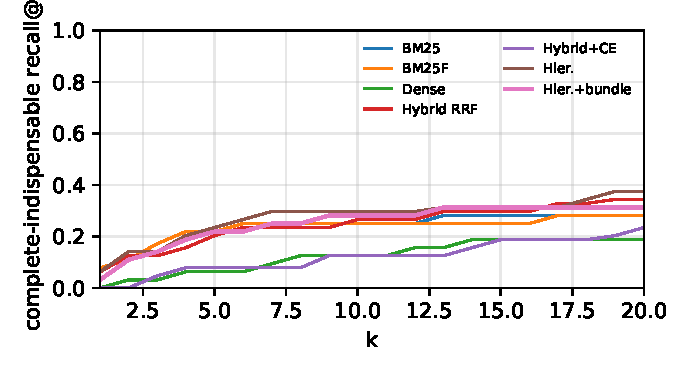
\includegraphics[width=\linewidth]{complete_at_k}
  \end{minipage}\hfill
  \begin{minipage}[c]{0.52\linewidth}
    \centering
    \scriptsize
    \begin{tabular*}{\linewidth}{@{\extracolsep{\fill}}lccc}
\toprule
Variant & C@10 & C@20 & R@20 \\
\midrule
Full system & 0.281 & 0.312 & 0.480 \\
\quad without expansion & 0.281 & 0.281 & 0.452 \\
\quad without act routing & 0.297 & 0.297 & 0.518 \\
\quad without field weights & 0.281 & 0.312 & 0.470 \\
\quad without dense & 0.281 & 0.281 & 0.439 \\
\quad without temporal & 0.281 & 0.344 & 0.496 \\
\quad without defines & 0.281 & 0.312 & 0.480 \\
\quad without excepts qualifies & 0.281 & 0.312 & 0.473 \\
\quad without xref procedural & 0.281 & 0.312 & 0.475 \\
\quad without amends & 0.281 & 0.281 & 0.465 \\
\quad without rerank & 0.281 & 0.281 & 0.454 \\
\bottomrule
\end{tabular*}

  \end{minipage}
  \caption{Left: complete-indispensable recall against the cutoff $k$ on the test split. The curves of the hybrid and hierarchical systems cross repeatedly and none clears 0.4 at $k=20$. Right: ablations of S7 (matter-macro means); no removal changes C@20 by more than one question in 32 matters.}
  \label{fig:curve}
\end{figure}

Removing Act routing raises R@20 (0.518 against 0.480) while lowering C@20 by
half a point. Removing the temporal filter raises C@20 to 0.344 because of one
question: its gold cites a section of a 2022 amending Act that recites the
2019 wording of a rule the consolidated text no longer carries, so the filter
that removes anachronistic law removes the only copy of the applicable text.

\section{Confidence intervals}
\label{app:ci}
\small
\begin{tabular}{lcccc}
\toprule
System & R@20 & C@10 & C@20 & MRR \\
\midrule
BM25 & 0.49 [0.35, 0.62] & 0.25 [0.09, 0.41] & 0.28 [0.12, 0.44] & 0.50 [0.36, 0.65] \\
BM25F & 0.48 [0.35, 0.61] & 0.25 [0.09, 0.41] & 0.28 [0.12, 0.44] & 0.54 [0.38, 0.70] \\
Dense & 0.38 [0.25, 0.50] & 0.12 [0.03, 0.25] & 0.19 [0.06, 0.34] & 0.32 [0.19, 0.45] \\
Hybrid RRF & 0.55 [0.41, 0.68] & 0.27 [0.12, 0.42] & 0.34 [0.19, 0.50] & 0.54 [0.40, 0.69] \\
Hybrid + CE & 0.41 [0.29, 0.54] & 0.12 [0.03, 0.23] & 0.23 [0.11, 0.39] & 0.22 [0.14, 0.32] \\
Hierarchical & 0.50 [0.34, 0.64] & 0.30 [0.16, 0.45] & 0.38 [0.22, 0.53] & 0.51 [0.35, 0.66] \\
Hier. + bundle & 0.48 [0.34, 0.63] & 0.28 [0.12, 0.44] & 0.31 [0.16, 0.47] & 0.50 [0.36, 0.64] \\
\bottomrule
\end{tabular}

\medskip

Paired matter-level bootstrap differences, S7 minus the named system (95\% CI), for complete recall at 20 and indispensable recall at 20:
\begin{itemize}\setlength{\itemsep}{0pt}
\item vs BM25: $\Delta$C@20 +0.031 [-0.062, +0.125], $\Delta$R@20 -0.011 [-0.100, +0.076]
\item vs BM25F: $\Delta$C@20 +0.031 [-0.062, +0.125], $\Delta$R@20 -0.002 [-0.092, +0.084]
\item vs Dense: $\Delta$C@20 +0.125 [+0.031, +0.250], $\Delta$R@20 +0.101 [-0.018, +0.229]
\item vs Hybrid RRF: $\Delta$C@20 -0.031 [-0.156, +0.078], $\Delta$R@20 -0.065 [-0.156, +0.026]
\item vs Hybrid + CE: $\Delta$C@20 +0.078 [-0.062, +0.234], $\Delta$R@20 +0.068 [-0.040, +0.187]
\item vs Hierarchical: $\Delta$C@20 -0.062 [-0.156, -0.000], $\Delta$R@20 -0.016 [-0.060, +0.021]
\end{itemize}


\section{Statutes in the corpus}
\label{app:statutes}
Table~\ref{tab:principal} lists every principal enactment in the frozen
corpus (fingerprint \texttt{\corpusFingerprint}) with the number of amending
Acts the corpus holds for it. The enactments are the \nPrincipal{} statutes
named in the Sri Lanka Law College conveyancing course tables, which rank
them in three categories; the amending Acts are those whose own text was
available as a separate document, so the count reflects source availability,
not the full amendment history.
% generated by scripts/statutory-qa/make_statute_table.py; do not edit
\footnotesize
\begin{longtable}{p{0.50\linewidth}crrrl}
\caption{Principal enactments in the frozen corpus (52), by year. Cat.\ is the curriculum category assigned by the Sri Lanka Law College conveyancing course tables (1 most important, 3 important). Sections are the retrieval units the parser produced. Amend.\ is the number of amending Acts held in the corpus as separate documents whose \textsc{amends} edges point to the enactment (60 in total, of which 9 record no target and are not counted). Fold.\ is the number of amending instruments already folded into the consolidated text. Edition is the text the section tree was built from.}\label{tab:principal}\\
\toprule Enactment & Cat. & Sections & Amend. & Fold. & Edition \\ \midrule \endfirsthead
\toprule Enactment & Cat. & Sections & Amend. & Fold. & Edition \\ \midrule \endhead
\bottomrule \endfoot
Prevention of Frauds Ordinance No. 7 of 1840 & 1 & 19 & 2 & 5 & consolidated \\
State Lands Encroachments Ordinance No. 12 of 1840 & 3 & 10 & 0 & 3 & consolidated \\
Definition of Boundaries Ordinance No. 1 of 1844 & 2 & 14 & 0 & 5 & consolidated \\
Wills Ordinance No. 21 of 1844 & 1 & 7 & 1 & 5 & consolidated \\
Deeds and Documents (Execution before Public Officers) Ordinance No. 17 of 1852 & 1 & 7 & 0 & 1 & consolidated \\
Land Surveys Ordinance No. 4 of 1866 & 3 & 7 & 0 & 1 & consolidated \\
Sannases and Old Deeds Ordinance No. 6 of 1866 & 3 & 10 & 0 & 1 & consolidated \\
Prescription Ordinance No. 22 of 1871 & 1 & 15 & 1 & 2 & consolidated \\
Matrimonial Rights and Inheritance Ordinance No. 15 of 1876 & 1 & 36 & 0 & 1 & consolidated \\
Lands Resumption Ordinance No. 4 of 1887 & 3 & 17 & 0 & 3 & consolidated \\
Civil Procedure Code No. 2 of 1889 & 1 & 798 & 0 & 55 & consolidated \\
Surveyors Ordinance No. 15 of 1889 & 3 & 20 & 0 & 6 & consolidated \\
Powers of Attorney Ordinance No. 4 of 1902 & 1 & 17 & 3 & 6 & consolidated \\
Notaries Ordinance No. 1 of 1907 & 1 & 42 & 5 & 19 & consolidated \\
Jaffna Matrimonial Rights and Inheritance Ordinance No. 1 of 1911 & 1 & 40 & 0 & 1 & consolidated \\
Trusts Ordinance No. 9 of 1917 & 3 & 123 & 1 & 5 & consolidated \\
Kandyan Succession Ordinance No. 23 of 1917 & 1 & 4 & 0 & 0 & consolidated \\
Registration of Documents Ordinance No. 23 of 1927 & 1 & 50 & 5 & 15 & consolidated \\
Muslim Intestate Succession Ordinance No. 10 of 1931 & 1 & 4 & 0 & 0 & consolidated \\
Buddhist Temporalities Ordinance No. 19 of 1931 & 2 & 44 & 1 & 11 & consolidated \\
Land Settlement Ordinance No. 20 of 1931 & 3 & 33 & 1 & 4 & consolidated \\
State Land (Claims) Ordinance No. 21 of 1931 & 3 & 7 & 0 & 0 & consolidated \\
Land Development Ordinance No. 19 of 1935 & 2 & 143 & 0 & 13 & consolidated \\
Bank of Ceylon Ordinance No. 53 of 1938 & 3 & 59 & 0 & 13 & consolidated \\
Urban Councils Ordinance No. 61 of 1939 & 3 & 263 & 0 & 48 & consolidated \\
Land Registers (Reconstructed Folios) Ordinance No. 18 of 1945 & 2 & 9 & 0 & 1 & consolidated \\
Town and Country Planning Ordinance No. 13 of 1946 & 3 & 95 & 1 & 5 & consolidated \\
State Lands Ordinance No. 8 of 1947 & 3 & 113 & 0 & 2 & consolidated \\
Municipal Councils Ordinance No. 29 of 1947 & 3 & 349 & 0 & 42 & consolidated \\
Registration of Old Deeds and Instruments Ordinance No. 35 of 1947 & 3 & 12 & 0 & 0 & consolidated \\
Thesawalamai Pre-emption Ordinance No. 59 of 1947 & 1 & 14 & 0 & 0 & consolidated \\
Mortgage Act No. 6 of 1949 & 2 & 126 & 0 & 6 & consolidated \\
Land Acquisition Act No. 9 of 1950 & 2 & 73 & 3 & 7 & consolidated \\
National Housing Act No. 37 of 1954 & 3 & 125 & 1 & 6 & consolidated \\
Tea and Rubber Estates (Control of Fragmentation) Act No. 2 of 1958 & 1 & 29 & 1 & 1 & as enacted \\
People's Bank Act No. 29 of 1961 & 3 & 63 & 3 & 7 & consolidated \\
Local Authorities Housing Act No. 14 of 1964 & 3 & 14 & 1 & 1 & consolidated \\
Nindagama Lands Act No. 30 of 1968 & 3 & 30 & 0 & 0 & consolidated \\
Land Reform Law No. 1 of 1972 & 2 & 83 & 4 & 5 & consolidated \\
Apartment Ownership Law No. 11 of 1973 & 1 & 50 & 3 & 4 & consolidated \\
State Mortgage and Investment Bank Law No. 13 of 1975 & 3 & 88 & 3 & 3 & consolidated \\
Urban Development Authority Law No. 41 of 1978 & 2 & 56 & 0 & 6 & consolidated \\
National Housing Development Authority Act No. 17 of 1979 & 3 & 91 & 5 & 5 & consolidated \\
Land Grants (Special Provisions) Act No. 43 of 1979 & 2 & 20 & 0 & 0 & consolidated \\
Stamp Duty Act No. 43 of 1982 & 1 & 75 & 0 & 10 & consolidated \\
Western Province Financial Statute No. 6 of 1990 & 1 & 108 & 0 & 0 & consolidated \\
Registration of Title Act No. 21 of 1998 & 1 & 75 & 0 & 0 & unconfirmed \\
Survey Act No. 17 of 2002 & 3 & 68 & 0 & 0 & as enacted \\
Stamp Duty (Special Provisions) Act No. 12 of 2006 & 1 & 16 & 1 & 1 & consolidated \\
Companies Act No. 7 of 2007 & 1 & 534 & 1 & 1 & consolidated \\
Land (Restrictions on Alienation) Act No. 38 of 2014 & 1 & 26 & 2 & 2 & consolidated \\
Revocation of Irrevocable Deeds of Gift on the Ground of Gross Ingratitude Act No. 5 of 2017 & 1 & 7 & 0 & 0 & as enacted \\
\end{longtable}


\end{document}
